\subsection{Problem Formulation}
Let $x$ denote a text prompt and let $y=(y_1,\ldots,y_T)$ denote the discrete
motion-token sequence obtained from a pretrained VQ-VAE tokenizer. T2M-GPT
models the conditional distribution
\begin{equation}
    p_{\theta}(y\mid x)=\prod_{t=1}^{T}p_{\theta}(y_t\mid y_{<t}, x),
\end{equation}
where the text condition is produced by a CLIP text encoder and the motion
tokens are predicted autoregressively. COMPASS fine-tunes the autoregressive
generator rather than replacing the VQ-VAE or the decoding pipeline.

A training example is $(x,x',y,r,m)$: $x'$ is a paired prompt,
$r\in\{\mathrm{preserve},\mathrm{alter}\}$ is its relation to $x$, and $m$
marks edited text positions. Preserving pairs retain the original action
semantics. Altering pairs change one action, direction, or body-part slot.
For either relation, $y$ is the original motion used to compute attribution;
for an altering pair it is not an edited-motion target. The broader motivation
includes speed, count, and temporal order, but these factors are not separately
evaluated here. Relation labels specify whether the prompt-pair objective
should encourage agreement or edit-local sensitivity.

\subsection{Framework Overview}
Figure~\ref{fig:framework} summarizes the T2M-GPT-family implementation.
The trainable modules are the autoregressive Transformer, including its output
head, an auxiliary projection $\phi$, and a predictor $q$. The source models
studied here freeze CLIP and the VQ-VAE; subsequent text-only adaptation is a
separate stage described in Section~\ref{sec:independent_adaptation}.
A teacher Transformer is initialized from the same pretrained checkpoint as
the student and remains frozen.

Each mini-batch contributes a generation loss on the original prompts. When
attribution objectives are active, both prompts are encoded and scored against
the original motion tokens. The relation label selects preserving alignment
or altering difference/locality losses. A frozen teacher regularizes the
resulting training objective. The auxiliary heads
are used only during training, so the motion vocabulary, tokenizer, and
inference architecture remain unchanged.

% TODO(figure): regenerate sato++.png. The current raster still draws the
% variance and covariance panels in the preserve branch, which were removed
% from the objective. The caption below flags this until the image is redrawn.
\begin{figure*}[t]
\centering
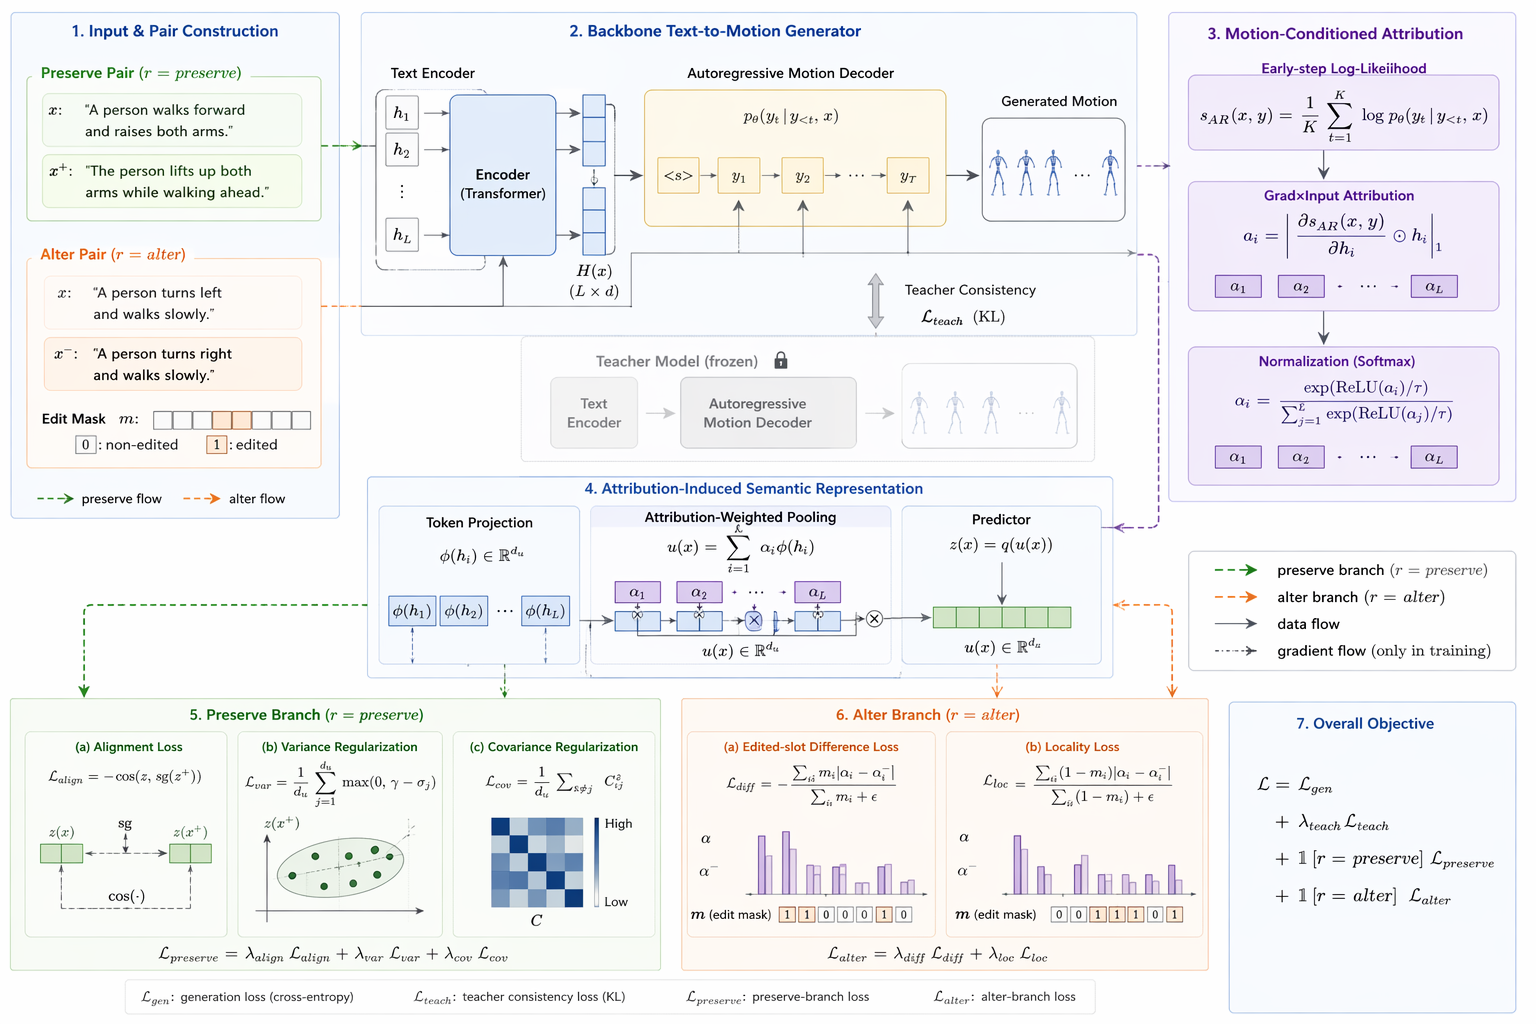
\includegraphics[width=\linewidth]{sato++.png}
\caption{COMPASS training framework. Early target-motion likelihoods provide
Grad~$\times$~Input weights for auxiliary text representations. Preserving
pairs use attribution-weighted alignment; altering pairs
use edited-position differences and unedited-position locality. A frozen
teacher constrains prediction drift. The schematic's KL teacher label applies
to the Motion-X MotionGPT preserve-only variant; T2M-GPT-family sources use
L1 logit matching. The variance and covariance panels drawn in the preserve
branch are not part of the objective reported here.
Attribution-gradient connectivity is configuration dependent.}
\label{fig:framework}
\end{figure*}

\subsection{Motion-Conditioned Token Attribution}
We derive token weights from the generator's likelihood of a particular target
motion. For prompt $x$ and motion tokens $y$, the attribution score averages
the first $K$ autoregressive predictions:
\begin{equation}
    s_{\mathrm{AR}}(x,y)=
    \frac{1}{K}\sum_{t=1}^{K}\log p_{\theta}(y_t\mid y_{<t},x),
\end{equation}
where $K$ is restricted to valid target-token positions. Let $h_i$ denote the
input CLIP token embedding at position $i$, distinct from the generator hidden
state $h_\theta$ used later. Grad~$\times$~Input assigns
\begin{equation}
    a_i(x,y)=
    \left\lVert
    \frac{\partial s_{\mathrm{AR}}(x,y)}{\partial h_i}\odot h_i
    \right\rVert_1 .
\end{equation}
The raw attribution values are converted into a probability distribution over
text positions:
\begin{equation}
    \alpha_i(x,y)=
    \frac{\exp(\mathrm{ReLU}(a_i)/\tau)}
    {\sum_j \exp(\mathrm{ReLU}(a_j)/\tau)} ,
\end{equation}
where $\tau$ is a temperature. Because the score is a target-motion likelihood,
$\alpha$ weights textual evidence relevant to that motion under the current
model. It is a local attribution measure, not a ground-truth importance label.
The distinction between differentiating through these weights and treating
them as constants is specified below.

\subsection{Attribution-Weighted Semantic Representation}
COMPASS pools token features with the attribution distribution:
\begin{equation}
    u(x,y)=\sum_i \alpha_i(x,y)\,\phi(H_i(x)),
\end{equation}
where $H_i(x)$ is the contextual CLIP feature and $\phi$ projects it into the
auxiliary representation space. A predictor produces
\begin{equation}
    z(x,y)=q(u(x,y)).
\end{equation}
The predictor is used for preserving alignment, following the stop-gradient
Siamese formulation~\cite{chen2021exploring}.

\subsection{Preserving Branch}
For $r=\mathrm{preserve}$, the paired prompts should describe the same target
motion even if they use different surface forms. COMPASS aligns their
motion-conditioned representations with a stop-gradient cosine objective:
\begin{equation}
    \mathcal{L}_{\mathrm{align}}
    =-\cos\bigl(z(x,y),\mathrm{sg}(z(x',y))\bigr),
\end{equation}
where $\mathrm{sg}(\cdot)$ denotes stop-gradient. The preserving objective
weights this alignment term:
\begin{equation}
    \mathcal{L}_{\mathrm{pres}}
    =
    \lambda_{\mathrm{align}}\mathcal{L}_{\mathrm{align}} .
\end{equation}
Cosine alignment alone admits a constant-representation solution. The
stop-gradient asymmetry between the two branches is the only structural
constraint against it here, and it does not guarantee that collapse is
avoided.

\subsection{Altering Branch}
For $r=\mathrm{alter}$, the edited slot should remain influential. Let
$m_i\in\{0,1\}$ indicate whether token position $i$ belongs to the edited slot.
COMPASS encourages attribution to change on edited positions:
\begin{equation}
    \mathcal{L}_{\mathrm{diff}}
    =
    -
    \frac{\sum_i m_i|\alpha_i(x,y)-\alpha_i(x',y)|}
    {\sum_i m_i+\epsilon}.
\end{equation}
The negative sign means that minimizing this term increases attribution
difference on the edited slot. At the same time, COMPASS penalizes attribution
drift outside the edited slot:
\begin{equation}
    \mathcal{L}_{\mathrm{loc}}
    =
    \frac{\sum_i (1-m_i)|\alpha_i(x,y)-\alpha_i(x',y)|}
    {\sum_i (1-m_i)+\epsilon}.
\end{equation}
The altering objective is
\begin{equation}
    \mathcal{L}_{\mathrm{alter}}
    =
    \lambda_{\mathrm{diff}}\mathcal{L}_{\mathrm{diff}}
    +
    \lambda_{\mathrm{loc}}\mathcal{L}_{\mathrm{loc}} .
\end{equation}
The negative sign rewards differences at edited positions, while the locality
term penalizes differences elsewhere. These losses specify a desired
attribution response to semantic edits; motion-level compliance requires
separate evaluation.

\subsection{Teacher-Preserved Fine-Tuning Objective}
The base generation loss is the T2M-GPT cross-entropy over target motion tokens,
\begin{equation}
    \mathcal{L}_{\mathrm{gen}}
    =
    -\sum_{t=1}^{T}\log p_{\theta}(y_t\mid y_{<t},x).
\end{equation}
To protect generation quality during robustness fine-tuning, the student is
regularized toward a frozen teacher. In the main T2M-GPT-family result reported
here, this teacher term is an L1 distance between student and teacher logits over
valid motion-token positions:
\begin{equation}
    \mathcal{L}_{\mathrm{teach}}
    =
    \frac{1}{T}\sum_t
    \left\lVert \ell_{\theta,t}-\ell_{\mathrm{teacher},t}\right\rVert_1 .
\end{equation}
The overall COMPASS loss is
\begin{equation}
    \mathcal{L}
    =
    \mathcal{L}_{\mathrm{gen}}
    +\lambda_{\mathrm{teach}}\mathcal{L}_{\mathrm{teach}}
    +\mathbf{1}_{r=\mathrm{preserve}}\mathcal{L}_{\mathrm{pres}}
    +\mathbf{1}_{r=\mathrm{alter}}\mathcal{L}_{\mathrm{alter}} .
\end{equation}
This equation describes the T2M-GPT-family objective used for the main COMPASS
checkpoints.  The MotionGPT plug-in reported in
Table~\ref{tab:motionx_methods} is a distinct preserve-only variant: it adds
paired-caption generation loss on $x'$, uses a KL teacher term, retains the
preserving alignment term, and sets the altering loss
weights to zero.  We therefore do not use that row as evidence for the full
preserve-plus-alter objective.

\subsection{Implementation and Gradient Paths}
The T2M-GPT-family source configurations use $K=16$, frozen CLIP and VQ-VAE
weights, L1 teacher matching, and
\texttt{attribution\_create\_graph=false}. Edit masks are mapped from annotated
words to CLIP positions. Detaching the score gradient removes the
second-order path through attribution. With CLIP also frozen, the attribution
objectives update auxiliary heads but have no direct gradient path to the
generator in the audited implementation. Generation and teacher losses supply
the generator updates (Section~\ref{sec:detail_attribution_details}).
The Motion-X MotionGPT preserve-only variant enables the attribution graph
and uses its own native text and motion components. We retain these
implementation distinctions when interpreting both the theory and results.

\subsection{Conditional Theory of Preserving-Prompt Robustness}
\label{sec:robustness_theory}
We separate the geometry of a consistency loss, the conditions under which
its update can improve a generator, and the consequences of hidden-state
stability for output probabilities. These are local, conditional statements,
not an assumption that the detached implementation satisfies their premises.

\paragraph{Local coordinates and hidden-state geometry.}
Fix target tokens, teacher-forced prefixes, text positions, and attention
masks. Let $e$ concatenate visible continuous text embeddings and $h_\theta(e)$
concatenate final generator states over fixed valid motion positions. Its
Euclidean norm corresponds to the Frobenius norm used in our diagnostics.
Let $\delta$ be a perturbation in these embedding coordinates and let
$\mathcal U_{\rm pres}$ be the local subspace spanned by embedded preserving
prompt differences. Its span need not consist entirely of valid semantic
edits. We assume twice continuously differentiable maps with bounded
derivatives on the analyzed neighborhood and nonzero basepoint norms for
both hidden and auxiliary representations. These assumptions exclude
nondifferentiable points of the attribution map; finite token replacements
need not satisfy the small-perturbation approximation. Define
\begin{equation}
\begin{aligned}
 r_\theta(e,\delta)&=\frac{\|h_\theta(e+\delta)-h_\theta(e)\|_2}
 {\|h_\theta(e)\|_2},\\
 \widetilde J_\theta&=\frac{\partial h_\theta(e)/\partial e}{\|h_\theta(e)\|_2}.
\end{aligned}
\label{eq:theory_relative_jacobian}
\end{equation}
The denominator is held fixed: $\widetilde J$ is not the Jacobian of
$h/\|h\|$. Taylor expansion gives
\begin{equation}
 r_\theta^2=\delta^\top\widetilde J_\theta^\top\widetilde J_\theta\delta
 +O(\|\delta\|_2^3).
\label{eq:theory_local_response}
\end{equation}
For class $c$ at basepoint $e$, let $S_c=\mathbb E[\delta\delta^\top\mid e,c]$.
The identity $v^\top Av=\operatorname{tr}(Avv^\top)$ yields
\begin{equation}
 \mathbb E[r_\theta^2\mid e,c]
 =\operatorname{tr}(\widetilde J_\theta S_c\widetilde J_\theta^\top)
 +O(\mathbb E[\|\delta\|_2^3\mid e,c]).
\label{eq:theory_trace}
\end{equation}
For centered perturbations $S_c$ is the covariance; otherwise it also
includes the mean outer product. Different token classes therefore probe
different directions of a common local map.

\paragraph{Proposition 1: the forward value of cosine alignment.}
Set $\bar z=z/\|z\|_2$ and $J_{\bar z}=\partial\bar z/\partial e$ with
$y$ fixed. The preserving loss satisfies
\begin{equation}
\begin{aligned}
 1+\mathcal L_{\rm align}
 &=\tfrac12\|\bar z(e+\delta,y)-\bar z(e,y)\|_2^2\\
 &=\tfrac12\delta^\top J_{\bar z}^\top J_{\bar z}\delta
 +O(\|\delta\|_2^3).
\end{aligned}
\label{eq:theory_alignment}
\end{equation}
\emph{Proof.} Unit vectors obey $\|a-b\|_2^2=2-2a^\top b$.
Substitute $\bar z(e+\delta)=\bar z(e)+J_{\bar z}\delta+O(\|\delta\|^2)$.
Its expectation is one half of
$\operatorname{tr}(J_{\bar z}S_{\rm pres}J_{\bar z}^\top)$ to leading order.
The loss value thus measures data-dependent projected Jacobian energy.
Stop-gradient preserves this value but changes its parameter derivative:
this is not an equivalence between the actual detached update and gradient
descent on a fully differentiated Jacobian penalty~\cite{chen2021exploring}.

For the differentiable forward pooling map, the chain rule gives
\begin{equation}
 J_u=\sum_i\alpha_i J_{\phi\circ H_i}
 +\sum_i\phi(H_i)(\nabla_e\alpha_i)^\top.
\label{eq:theory_pooling_jacobian}
\end{equation}
Motion-conditioned weights allocate sensitivity according to the current
model's target-likelihood evidence, not ground-truth semantic importance.
Retaining the attribution-gradient graph can introduce mixed second
likelihood derivatives; detaching it removes this path while leaving any
remaining trainable feature/head paths. Consistent normalized attribution
maps alone do not bound the magnitude of the underlying input gradient.

Small $J_{\bar z}$ does not automatically imply small generator Jacobian
$J_h$. A sufficient additional bridge is
\begin{equation}
 \|J_h v\|_2\le\kappa\|J_{\bar z}v\|_2,
 \qquad v\in\mathcal U_{\rm pres}.
\label{eq:theory_bridge}
\end{equation}
For instance, this holds if the relevant local map factors as $h=f(\bar z)$
with $\|J_f\|_2\le\kappa$; merely sharing parameters is insufficient.
Then expected squared hidden drift is bounded by
$2\kappa^2\mathbb E[1+\mathcal L_{\rm align}]$ plus a third-order remainder.
We do not assume this factorization for COMPASS's auxiliary pooling head.

\paragraph{Proposition 2: sufficient cross-class contraction.}
Let subscripts $0,+$ denote the parent and COMPASS at the same input and
prefixes. Suppose that on $\mathcal U_{\rm pres}$,
\begin{equation}
 \widetilde J_+^\top\widetilde J_+
 \preceq\gamma^2\widetilde J_0^\top\widetilde J_0,
 \qquad 0<\gamma<1.
\label{eq:theory_contraction}
\end{equation}
Then $r_+\le\gamma r_0+O(\|\delta\|_2^2)$ for every sufficiently small
direction in the subspace. Expected squared responses satisfy the analogous
bound with factor $\gamma^2$, up to a third-order remainder, for each class
supported there. \emph{Proof.} The positive-semidefinite ordering bounds
$\|\widetilde J_+\delta\|_2$ by $\gamma\|\widetilde J_0\delta\|_2$;
Taylor expansion and the triangle inequality give the response bound, and
\eqref{eq:theory_trace} gives its expectation. Approximate proportionality
$\widetilde J_+\approx\gamma Q\widetilde J_0$, $Q^\top Q=I$, is a stronger
possible explanation for similar relative reductions across classes.
Neither similar class means nor smaller individual spectral norms establish
the directional ordering in~\eqref{eq:theory_contraction}.

\paragraph{Proposition 3: conditional risk reduction by an attribution update.}
Let $\theta_g$ contain only generator parameters, with auxiliary parameters
fixed during the comparison. Let $R(\theta_g)$ be a differentiable average
risk under a fixed preserving-perturbation distribution, such as perturbed
cross-entropy or $\mathbb E[r_\theta^2]$, rather than worst-case adversarial
risk. Let $a_g$ be the gradient delivered by the implemented attribution
objective to $\theta_g$, including stop-gradient choices, and
$b_g=\nabla_{\theta_g}R$. If $R$ is $\beta$-smooth along the update segment,
then for $\lambda>0$ and step size $\eta\ge0$,
\begin{equation}
\begin{aligned}
 R(\theta_g-\eta\lambda a_g)-R(\theta_g)
 \le{}&-\eta\lambda\langle b_g,a_g\rangle\\
 &+\tfrac12\beta\eta^2\lambda^2\|a_g\|_2^2.
\end{aligned}
\label{eq:theory_descent}
\end{equation}
\emph{Proof.} Apply the smoothness descent lemma with increment
$-\eta\lambda a_g$. Positive $\langle b_g,a_g\rangle$ ensures strict
reduction for sufficiently small steps. For $\beta>0$, it suffices that
$0<\eta<2\langle b_g,a_g\rangle/(\beta\lambda\|a_g\|_2^2)$.
This is an attribution-only Euclidean update, not a guarantee for a joint
Adam update, whose effective direction must be considered separately.
If $a_g=0$, the generator update is zero and its gradient cosine is undefined.
Our frozen-CLIP detached-attribution audit finds this disconnected case
(Section~\ref{sec:detail_attribution_details}); the strict-descent premise is
therefore unavailable for that configuration.

\paragraph{Proposition 4: conditional output-distribution bounds.}
At a shared autoregressive prefix $v$, write $h_t=h_{\theta,t}(e;v)$ and
$h_t'=h_{\theta,t}(e+\delta;v)$. Suppose
$\|\ell_t-\ell_t'\|_2\le M_t\|h_t-h_t'\|_2$ in the neighborhood;
for a linear head one may take $M_t=\|W_t\|_2$. Define the unit-temperature
probabilities $p_t=\operatorname{softmax}(\ell_t)$ and
$p_t'=\operatorname{softmax}(\ell_t')$. With $\operatorname{CE}$ denoting
cross-entropy and $D_{\rm KL}$ Kullback--Leibler divergence,
\begin{equation}
\begin{aligned}
 D_{\rm KL}(p_t\|p_t')&\le\tfrac14 M_t^2\|h_t-h_t'\|_2^2,\\
 |\operatorname{CE}(\ell_t',y_t)-\operatorname{CE}(\ell_t,y_t)|
 &\le\sqrt{2}M_t\|h_t-h_t'\|_2.
\end{aligned}
\label{eq:theory_output_bounds}
\end{equation}
\emph{Proof.} For $A(\ell)=\log\sum_j\exp(\ell_j)$,
$\nabla^2A=\operatorname{diag}(p)-pp^\top$ has spectral norm at most $1/2$.
Thus $D_{\rm KL}(p\|p')=D_A(\ell',\ell)\le\|\ell'-\ell\|_2^2/4$,
where $D_A$ is the Bregman divergence generated by $A$.
Also $\|\nabla_\ell\operatorname{CE}\|_2=\|p-e_{y_t}\|_2\le\sqrt2$,
where $e_{y_t}$ is the one-hot target vector.
For fixed horizon $T$ (or absorbing EOS padding), the KL chain rule yields
\begin{equation}
 D_{\rm KL}(P_e\|P_{e+\delta})
 \le\tfrac14\sum_{t=1}^T M_t^2
 \mathbb E_{v\sim P_e}[\|h_t-h_t'\|_2^2],
\label{eq:theory_sequence_kl}
\end{equation}
provided the bounds hold at every prefix in the expectation. Here $P_e$ is
the sequence law and both conditionals use the same sampled prefix $v$.
Measurements at selected target prefixes alone do not verify this premise.
Guidance requires bounds on its actual combined logits; truncation changes
the probability law. These statements do not certify individual sampled
trajectories or imply monotone FID, diversity, or retrieval gains. Comparing
models also requires accounting for their different head norms $M_t$.

\paragraph{Roles and limits of the remaining regularizers.}
By the triangle inequality, the student's prompt-pair logit difference is at
most the teacher's difference plus the two student--teacher residuals.
Teacher matching limits drift but does not guarantee improvement over the
teacher.
Altering losses prefer edit-local evidence changes, not a proven lower bound
on motion-level edit response. The theoretical scope is the evaluated
preserving-perturbation family, not global invariance or certified semantic
control.
